\chapter{Introduction}
\label{0}


% Adhesive advantages
Adhesive unions present themselves as a promising solution for bonding manufacture, thanks to their properties and last years improvements on these.

\begin{figure}
\centering
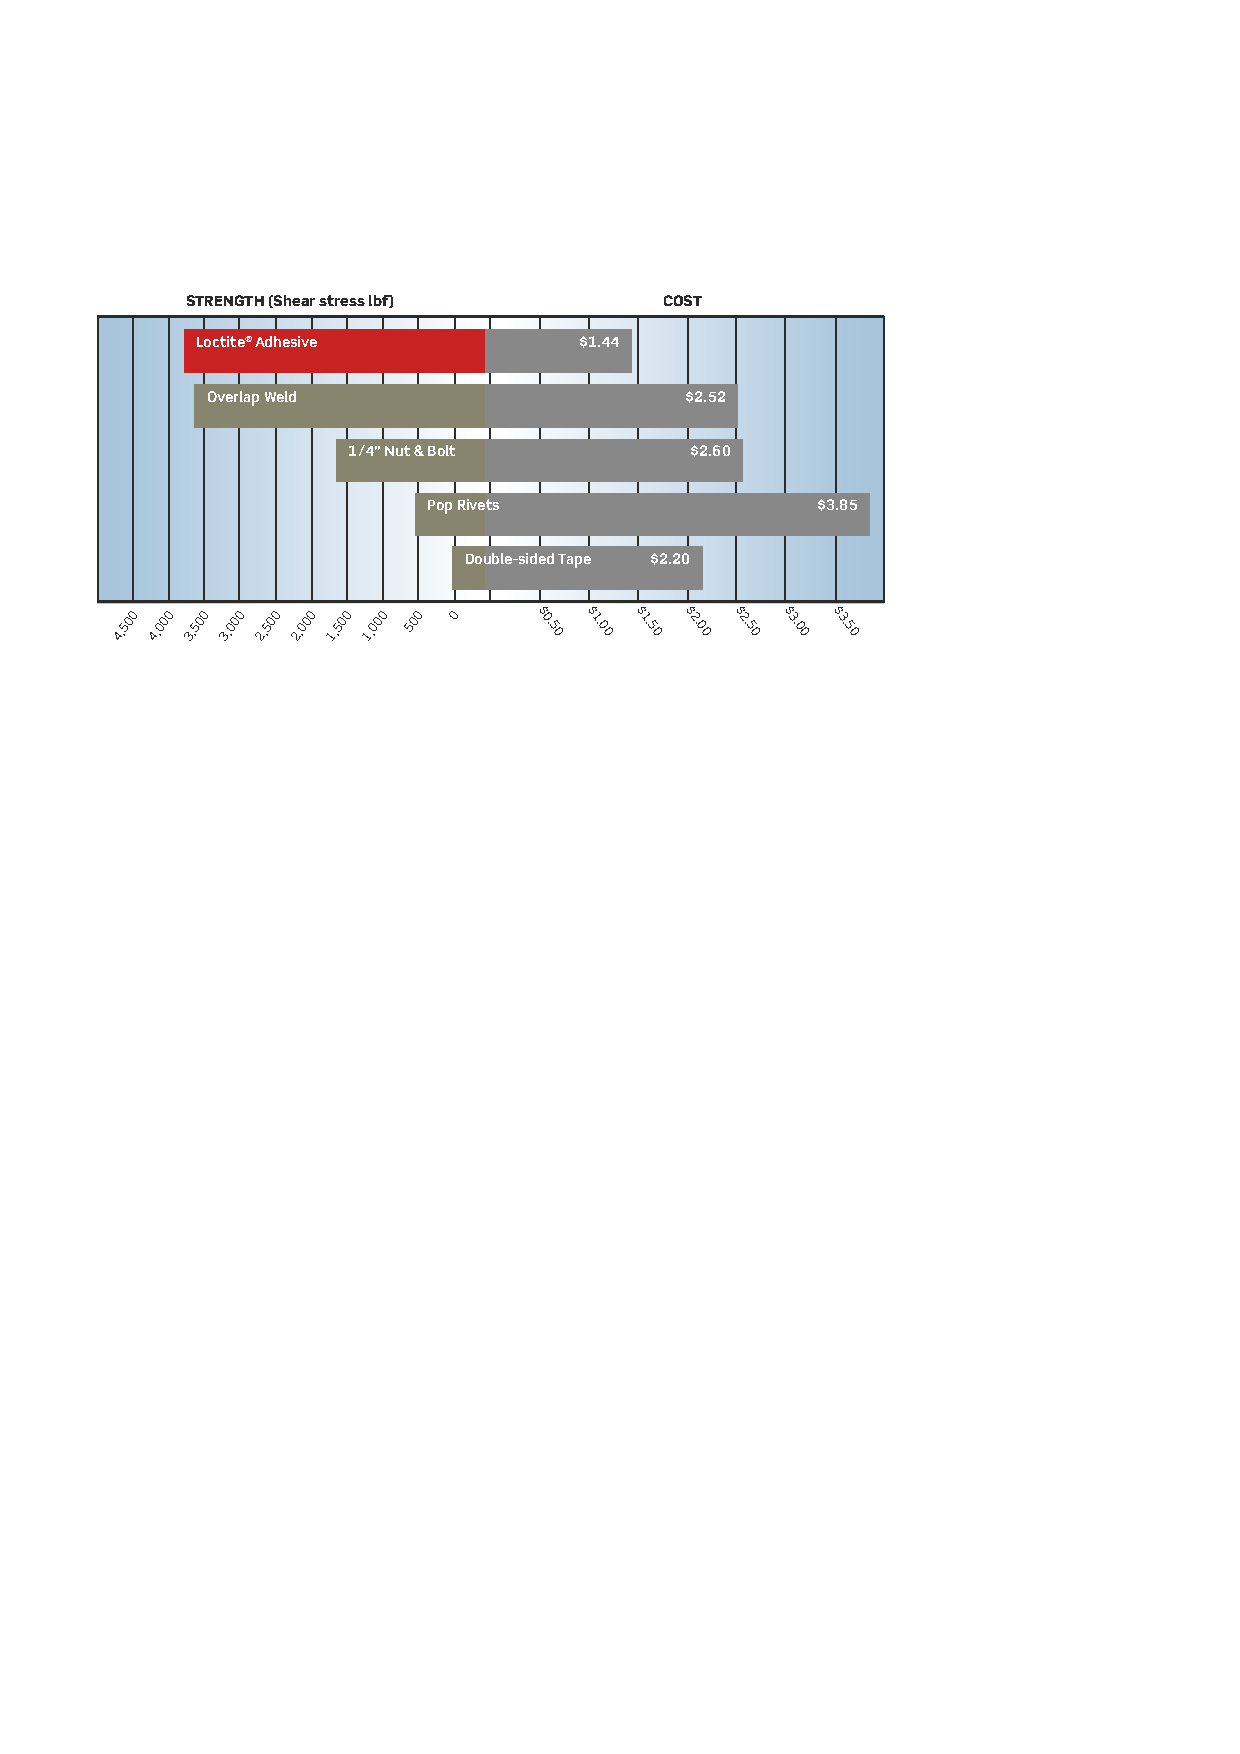
\includegraphics[angle=0,width=0.8\columnwidth]{comparison}
\caption{Qualitative strength and economical comparison of different bonding solutions. Taken from \citet{superyacht}}
\label{fig:comparison}
\end{figure}

As figure \ref{fig:comparison} illustrates, adhesives are very competitive both in bonding strength and in economical manufacture costs. Although other solutions, like welding, may compete in strength, adhesive are much more inexpensive than other solutions. It is recalled that this figure only aims to give an idea of this comparison, and should not be taken as a fact.

\section{Interesting adhesive properties}
% Resistance (general)
Advancements in the last years have improved adhesives resistant properties, making them competitive against other bonding solutions for certain applications. This improvements are especially remarkable on their peel resistance, which used to be one of the main obstacles for spreading their use in different industries. Conversely, shear resistance outstands when compared to other loading cases.
% Fatigue
Fatigue resistance is a key feature of this bonding, especially in certain mechanical applications, such as in structural unions in vehicles, aircrafts and machines, where vibrations suppose an important solicitation over time. They also provide certain damping \citep{Loureiro2010}, insulating other components from vibrations.

There are also different adhesive brands and solutions, providing a wide range of properties adapting to each case need, like allowing stiff and flexible bonds \citep{Loureiro2010}. Moreover, they can be improved with certain additives \citep{Vaidya2006}, although this may go against manufacturer recomendations in some cases.
% Brittleness
Adhesive unions have to be applied to larger areas ---if compared to other solutions, such as \gls{SW}--- and, although that is not an structural property, this allows a more continuous behaviour \citep{Vaidya2006, Liao2011} by contributing to load distribution and to \gls{Pk} reduction, resulting on a less brittle union on its ultimate state.
% Manufacture
The casting process also contributes on reducing brittleness: lower temperatures are required (if compared with welding) resulting in less damage to adherents’ properties, and great uniformity can be achieved in the union itself and between different unions. Manufacture easiness also allows the creation of hybrid unions, in which the properties of one type of bonding are improved by the use of another one in addition \citep{Sadowski2010, Sadowski2011}. They also allow the creation of bonds between adherends of different nature when needed \citep{Wu2013}, a feature that cannot be found on other bonding solutions, such as welded unions.
% Density
Among its non-structural properties, its reduced density is a remarkable step to create light weight unions with many different benefits, which vary between applications, but interesting both economically and environmentally. Recent changes on european regulations \citep{pistonudos} will make light-weight solutions even more important in the next years.

\section{Usage}
Due to mentioned properties ---but specially their resistance and light-weight---, adhesives have become a widely used bonding solution in the aerospatial industry: in fuselage structure, in aircraft wings stiffener ribs, etc.

It is also becoming an appealing bonding solution in others, such as in the automotive industry \citep{Wu2006, Greve2007, Grant2009, Scattina2011, Kadioglu2014, SernaMoreno2015}, where they are being used to cast more unions each moment.

Even other industries like the yachting one \citep{superyacht} are starting to implement this technology thanks to the adhesive durability, environmental impact, strength and manufacture costs.

\subsection{Crash boxes}
In the automotive industry, one of the latest applications of this bonding system is the use of adhesives in crash box design, and it is the focus of this study.

Crash boxes belong to the pasive safety measures installed on a vehicle. Pasive safety refers to minimizing damage to the occupants during an accident, being active safety a set of measures that aim to prevent the event itself.
% Introd to adhesive crash box
These devices are installed as a part of the vehicle's structure, usually just behind the bumper, being their function to absorb the most in case of impact on an accident. As an example, the precise location of these elements in a 2011 Audi A8 is showed in figure \ref{fig:audi_struc}, and detailed in figure \ref{fig:audi_detail}. In the general view, different materials are highlighted, illustrating how adhesives can be interesting in this industry.

\begin{figure}
\centering
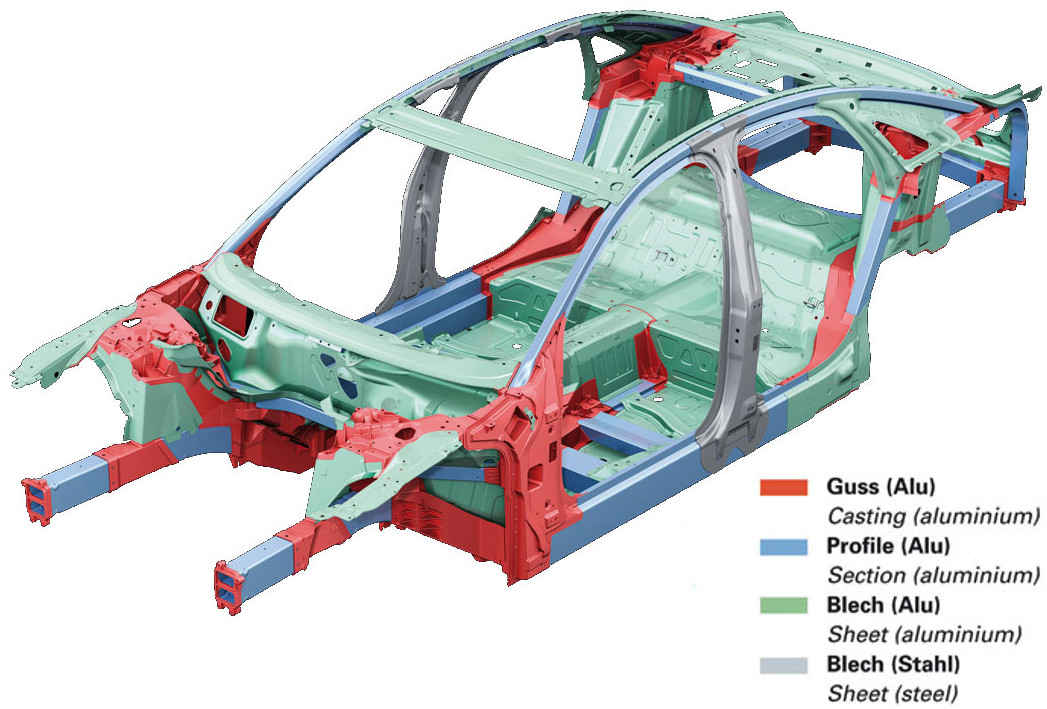
\includegraphics[angle=0,width=0.8\columnwidth]{audiA8struc}
\caption{Body structure of a 2011 Audi A8. Taken from \citet{phdCostas}}
\label{fig:audi_struc}
\end{figure}

\begin{figure}
\centering
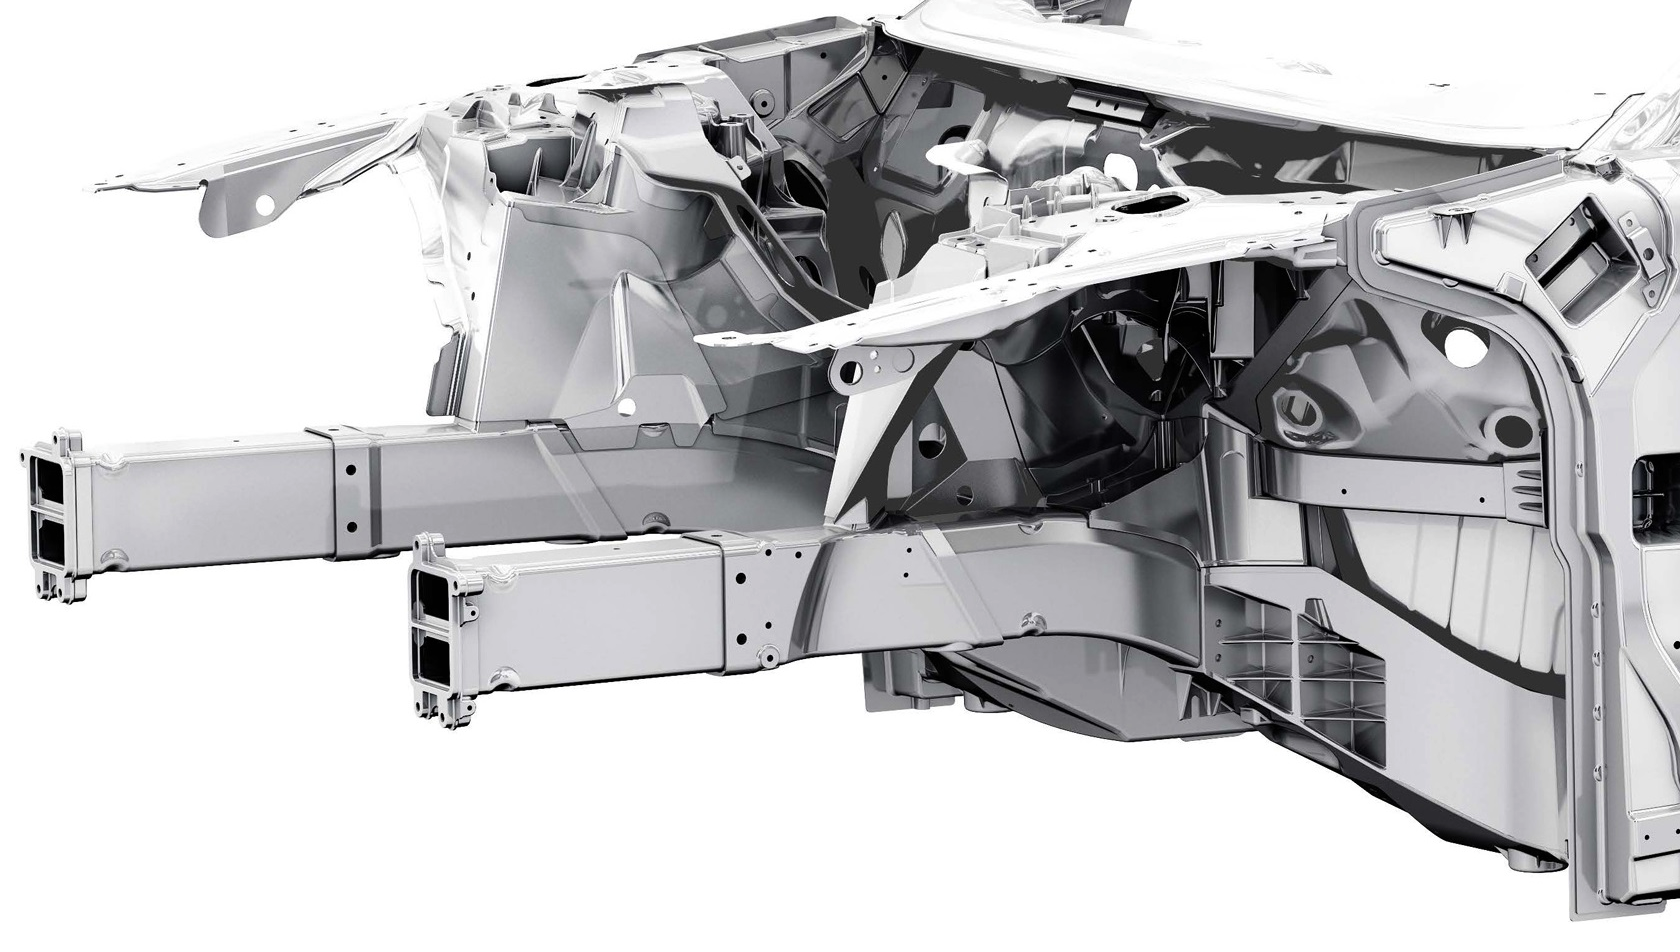
\includegraphics[angle=0,width=0.8\columnwidth]{audiA8detail}
\caption{Detail of energy absorption devices in the front of a 2011 Audi A8. In this case, an aluminum tube with two cavities was used. Taken from \citet{phdCostas}, original image copyrighted by Audi AG \citep{audi}}
\label{fig:audi_detail}
\end{figure}

% Design variables
As \citet{Hou2008} pointed, the design of a crashworthy element pursues to maximize \gls{Ea} through elastic and plastic deformation \citep{Wu2006}, but this also increases the \gls{Pk}, which is considered one of the main reasons of biomechanical injury. \Gls{SEA} has been used as parameter by some authors \citep{Lee2006, Peroni2009, Scattina2011} for measuring the element's effectiveness on absorving energy, rather than the total \gls{Ea}. A compromise between \gls{Ea} ---or \gls{SEA} on its place--- and \gls{Pk} has to be achieved. Weight is another variable usually taken into account.

\section{Literature review}

\subsection{Experiments on adhesives}
\citet{Lee2006} showed the adhesive's better performance if compared to \gls{SW} in terms of \gls{SEA}. These two bonding methods were also tested, toghether with \gls{LW}, by \citet{Peroni2009}, who also included different box section geometries in their studies.

On impact, a Charpy-like pendulum has been used to test adhesive behaviour \citep{Goglio2008, Kadioglu2014}. It was concluded that maximum stresses strongly vary when comparing to static results \citep{Goglio2008}. \citet{Kadioglu2014} tested adhesive tape and found that results vary very little with impact speed.

\subsubsection{\Gls{SLJ} and peel test}

Although different tests were proposed \citep{Kihara2003, Raykhere2010} in order to obtain adhesive's properties on peel and shear loading, \gls{SLJ} and peel test remain as the most extended experiments to obtain shear and traction stiffness and strength of different bonding solutions.

Many authors have tried variations on these tests \citep{Grant2009, Liao2011} in order to check the influence of different parameters, such as the adhesive layer thickness and overlap length, or including fillets on the bonding edges.

\citet{Loureiro2010} presented a very complete study of stiff and flexible adhesive's properties, in which they tested \gls{SLJ} and T-joints analyzing its mechanical behaviour on static, impact and fatigue loads, apart from damping measurement. They found that stiff adhesives had a bigger impact failure load than their counterpart, although they are comparable. In \glspl{SLJ}, stiff adhesives produced adherend yielding, which was the cause of the failure load increase. Flexible adhesives showed a bigger distribution in time of load and adherend yielding in T-joints.

\subsection{Modelling}

Adhesive bonding behaviour has been widelly modelled \citep{Sato2000, Alfano2001, Kihara2003, Vaidya2006, Wu2006, Hou2008, Grant2009, Peroni2009, Sadowski2010, Scattina2011, Sadowski2011, Liao2011, Yang2012}, usually as a previous phase to laboratory experiences, which usually included \glspl{SLJ} and peel tests.

The \gls{SLJ} test has also been modelled \citep{Vaidya2006}, as a way of obtaining its parameters for the used formulation \citep{Scattina2011}. Analogously, some authors used \glspl{SLJ} as a validation for their models \citep{Liao2011}. \Gls{SLJ} modelling allows many different analysis:
\begin{itemize}
\item Stress distribution over the bonded surface: this was the main focus of the study carried out by \citet{Liao2011}, finding a great uniformity if compared to other bonding solutions and highlighting the mostly stressed regions, which would help in reinforcements design if needed.
\item Comparison with other tests: like tapered lap and scarf joints modelled by \citet{Sato2000}.
\item Comparison with other bonding solutions: such as rivets and hybrid unions of rivets and adhesives \citep{Sadowski2010, Sadowski2011}.
\end{itemize}

In spite of having been modelled for long time, the adhesive behaviour formulation was not clear until recently. During the development of the formulation used nowadays, other models have been used, including: three and five elements Voigt viscoelastic models \citep{Sato2000}; isotropic elastic-plastic material with kinematic hardening \citep{Vaidya2006}; and even a highly specific formulation for this bonding system \citep{Greve2007}. Adhesives are nowadays modelled as linear elastic isotropic materials with damage models, being thus a case of \gls{LEFM}.

Eventually, formulation development lead to modelling of entire crash boxes \citep{Scattina2011, Yang2012, Yamashita2013}.

\citet{Sadowski2010, Sadowski2011, Sadowski2014} modelled hybrid unions with the use of rivets at different scales, and eventually tested crash boxes with hybrid bonds.

\section{Presentation of the study}
% Presentation of study
In order to check adhesive's suitability for their use in crashworthy elements, in the present study, numerical models of adhesively bonded crash boxes subjected to impact load have been developed using the \gls{FEM}. Information and data present in the literature are used to create and validate these models in order to ensure the accuracy of the results.

%------------------------------------------------
\citet{Kihara2003} made a two-dimensional analysis through the FEM in order to model their proposed experiment before taking it to the laboratory. On their experiments, they took special attention on the crack of the adhesive layer.

\citet{Vaidya2006} continued this studies by deeply analysing, numerically and experimentally, lap joints casted with adhesives on impact. They analysed the adhesive's response under different load types, including a peel and transverse loads combination, and tried the addition of nanoclay to the adhesive, resulting in an approximate 20\% Young's modulus and a decrease of the ultimate failure strain of one third of the original.

The energy absorption of this last mechanism in elastic-plastic materials was studied by \citet{Wu2006}, and compared it to the other mechanism of dissipation: plastic deformation. This was carried out with a 2D-model with axisymmetry, as the impact conditions allowed to do so, and taking special attention on the contact modelling. The restitution coefficient was also taken into account, as a measure of the amount of dissipated energy, relating it to the impact velocity.

The design of a crashworthiness element pursues to absorb the greatest amount of energy through deformation but, as \citet{Hou2008} showed, this also increases the peak force, which is considered one of the main reasons of biomechanical injury, becoming another key parameter in the design. These authors also analysed several multi-cell sections (up to a quadruple-cell section), showing their differences in their response. They made a multi-objective optimization, and a single-objective optimization taking other objectives as constrains, comparing the results.

\citet{Lee2006} tested double hat-shaped specimens with spot-welded with similar materials, and adhesively bonded with steel and aluminium. They found that both specimens absorbed aproximatedly the same energy, although the aluminium-steel adhesively bonded one had a 37\% increase of its specific energy absorption (SEA), in spite of a decrease of the mean crush load. They also made a point on the collapse modes of the adhesive and of the other bonding methods tested.

Using carbon fiber reinforced plastic (CFRP) adherends, \citet{Wu2013} analysed the crashworthiness of this adhesive joints under transverse loads. They tested the overlap length and width on the joint load, stiffness, propagation displacement and absorbed energy on quasi-static experiments. On impact, they analysed the relation of force with deflection and with time, and of the energy absorption with time and with impact energy. They found that the bigger the peak absorbed energy, the more proportion of energy was finally absorbed. A part of this energy was rebounded to the system. They also found force drops in their experiments, due to the initiation of the adhesive crack.

\citet{Peroni2009} compared the traditional joining technique in the automotive industry (spot-welding) to adhesive and laser joints, in order to show the aptitude of this two novel bonding methods. They presented the main adhesive's advantages and drawbacks, remarking that structural adhesives have improved their peel stress resistance, which used to be one of their main problems. In spite of this, triggers and rivets were practiced into the test boxes in order to ensure an stable collapse. They presented five experimental configurations (two flanged and three unflanged), and the key problems of each, with focus on manufacturing difficulties. The results were satisfactory: adhesive bonding gives a better performance than spot-wielding, and is comparable with laser bonding, which is slightly stiffer.

\citet{Greve2007} proposed a highly specific model for thin-layer high-strength adhesives. Certain phenomena, such as the non-conservation of volumen through deformation, make these new models necessary. A fracture criterion was token into account for this modelling, although more work in this field is needed, as stated. Two different FEM were simulated: one with solid elements for the adhesive, and another with node-to-element modelling. Both gave good results when compared to the real model, although the former gave the best adjustment, while the later had a much lower computational cost.
